% -*- Mode:TeX -*-

%% IMPORTANT: The official thesis specifications are available at:
%%            http://libraries.mit.edu/archives/thesis-specs/
%%
%%            Please verify your thesis' formatting and copyright
%%            assignment before submission.  If you notice any
%%            discrepancies between these templates and the 
%%            MIT Libraries' specs, please let us know
%%            by e-mailing thesis@mit.edu

%% The documentclass options along with the pagestyle can be used to generate
%% a technical report, a draft copy, or a regular thesis.  You may need to
%% re-specify the pagestyle after you \include  cover.tex.  For more
%% information, see the first few lines of mitthesis.cls. 

%\documentclass[12pt,vi,twoside]{mitthesis}
%%
%%  If you want your thesis copyright to you instead of MIT, use the
%%  ``vi'' option, as above.
%%
%\documentclass[12pt,twoside,leftblank]{mitthesis}
%%
%% If you want blank pages before new chapters to be labelled ``This
%% Page Intentionally Left Blank'', use the ``leftblank'' option, as
%% above. 

\documentclass[12pt,twoside]{mitthesis}
\usepackage{lgrind}
\usepackage{url}
\usepackage{acronym}
\usepackage[colorlinks=true,urlcolor=black,colorlinks=true,linkcolor=black,citecolor=black,filecolor=black,urlcolor=black,]{hyperref}
\usepackage{tabularx}
\usepackage{multirow}
\usepackage{fancyref}
\usepackage[gen]{eurosym}
%\usepackage[backend=bibtex,url=true]{biblatex} 
\pagestyle{plain}

%% This bit allows you to either specify only the files which you wish to
%% process, or `all' to process all files which you \include.
%% Krishna Sethuraman (1990).

%\typein [\files]{Enter file names to process, (chap1,chap2 ...), or `all' to
%process all files:}
%\def\all{all}
%\ifx\files\all \typeout{Including all files.} \else \typeout{Including only \files.} \includeonly{\files} \fi

\begin{document}

% -*-latex-*-
% 
% For questions, comments, concerns or complaints:
% thesis@mit.edu
% 
%
% $Log: cover.tex,v $
% Revision 1.8  2008/05/13 15:02:15  jdreed
% Degree month is June, not May.  Added note about prevdegrees.
% Arthur Smith's title updated
%
% Revision 1.7  2001/02/08 18:53:16  boojum
% changed some \newpages to \cleardoublepages
%
% Revision 1.6  1999/10/21 14:49:31  boojum
% changed comment referring to documentstyle
%
% Revision 1.5  1999/10/21 14:39:04  boojum
% *** empty log message ***
%
% Revision 1.4  1997/04/18  17:54:10  othomas
% added page numbers on abstract and cover, and made 1 abstract
% page the default rather than 2.  (anne hunter tells me this
% is the new institute standard.)
%
% Revision 1.4  1997/04/18  17:54:10  othomas
% added page numbers on abstract and cover, and made 1 abstract
% page the default rather than 2.  (anne hunter tells me this
% is the new institute standard.)
%
% Revision 1.3  93/05/17  17:06:29  starflt
% Added acknowledgements section (suggested by tompalka)
% 
% Revision 1.2  92/04/22  13:13:13  epeisach
% Fixes for 1991 course 6 requirements
% Phrase "and to grant others the right to do so" has been added to 
% permission clause
% Second copy of abstract is not counted as separate pages so numbering works
% out
% 
% Revision 1.1  92/04/22  13:08:20  epeisach

% NOTE:
% These templates make an effort to conform to the MIT Thesis specifications,
% however the specifications can change.  We recommend that you verify the
% layout of your title page with your thesis advisor and/or the MIT 
% Libraries before printing your final copy.
\title{Reengineering a Content Manager for Humanoid Robots with Web Technology}

\author{Eduard Gamonal Capdevila}
% If you wish to list your previous degrees on the cover page, use the 
% previous degrees command:
%       \prevdegrees{A.A., Harvard University (1985)}
% You can use the \\ command to list multiple previous degrees
%       \prevdegrees{B.S., University of California (1978) \\
%                    S.M., Massachusetts Institute of Technology (1981)}
\department{\Fib}

% If the thesis is for two degrees simultaneously, list them both
% separated by \and like this:
% \degree{Doctor of Philosophy \and Master of Science}
\degree{Master in Information Technology}

% As of the 2007-08 academic year, valid degree months are September, 
% February, or June.  The default is June.
\degreemonth{December}
\degreeyear{2013}
\thesisdate{Dec 18, 2013}

%% By default, the thesis will be copyrighted to MIT.  If you need to copyright
%% the thesis to yourself, just specify the `vi' documentclass option.  If for
%% some reason you want to exactly specify the copyright notice text, you can
%% use the \copyrightnoticetext command.  

\copyrightnoticetext{\copyright This work is licensed under the Creative Commons Attribution 4.0 International License. To view a copy of this license, visit \url{http://creativecommons.org/licenses/by/4.0/}.}

% If there is more than one supervisor, use the \supervisor command
% once for each.
%\supervisor{N\'{u}ria Castell Ari\~{n}o}

% This is the department committee chairman, not the thesis committee
% chairman.  You should replace this with your Department's Committee
% Chairman.
%\chairman{Daniel Pinyol}{CTO at \company}

% Make the titlepage based on the above information.  If you need
% something special and can't use the standard form, you can specify
% the exact text of the titlepage yourself.  Put it in a titlepage
% environment and leave blank lines where you want vertical space.
% The spaces will be adjusted to fill the entire page.  The dotted
% lines for the signatures are made with the \signature command.
\maketitle

% The abstractpage environment sets up everything on the page except
% the text itself.  The title and other header material are put at the
% top of the page, and the supervisors are listed at the bottom.  A
% new page is begun both before and after.  Of course, an abstract may
% be more than one page itself.  If you need more control over the
% format of the page, you can use the abstract environment, which puts
% the word "Abstract" at the beginning and single spaces its text.

%% You can either \input (*not* \include) your abstract file, or you can put
%% the text of the abstract directly between the \begin{abstractpage} and
%% \end{abstractpage} commands.

% First copy: start a new page, and save the page number.

\cleardoublepage
% Uncomment the next line if you do NOT want a page number on your
% abstract and acknowledgments pages.
\pagestyle{empty}
\setcounter{savepage}{\thepage}

\begin{abstractpage}

% $Log: abstract.tex,v $
% Revision 1.1  93/05/14  14:56:25  starflt
% Initial revision
% 
% Revision 1.1  90/05/04  10:41:01  lwvanels
% Initial revision
% 
%
%% The text of your abstract and nothing else (other than comments) goes here.
%% It will be single-spaced and the rest of the text that is supposed to go on
%% the abstract page will be generated by the abstractpage environment.  This
%% file should be \input (not \include 'd) from cover.tex.

This project aims at reengineering a content manager for humanoid robots with web technology at \company in order to abandon the current \flash implementation.
This software in the robot displays content applications and handles user interaction.

In the first part, this thesis describes the boundaries and context of the project and provides a general overview of related topics that support this work.

In the second part, this thesis addresses the reengineering of the software based on Pressman's work, in 6 steps: software inventory, documentation restructure and reverse engineering, code and data restructuring and forward engineering.

First it identifies the constraints of the project as well as its functional and non-functional requirements.

Secondly, it presents the specification emphasising the first 3 steps.
This work includes a conceptual model, system use cases and sequence diagrams.

Thirdly, it describes the internal design of the system in the context of the last 3 steps.
It starts by highlighting the system's architecture, its context and the software patterns.
Fourthly, it provides a static view with class and packages diagram, a dynamic view with sequence diagrams and a physical view with a deployment diagram.

The following chapter provides an overview of the most relevant parts of the implementation with code examples.

Finally, it outlines the testing strategy and explains the testing system's implementation.

In conclusion, this master's thesis addresses the development of the new system with accuracy and consistency and describes the construction of the software applying a systematic approach, proven techniques like software patterns and architectures, and creativity.



\end{abstractpage}

% Additional copy: start a new page, and reset the page number.  This way,
% the second copy of the abstract is not counted as separate pages.
% Uncomment the next 6 lines if you need two copies of the abstract
% page.
% \setcounter{page}{\thesavepage}
% \begin{abstractpage}
% % $Log: abstract.tex,v $
% Revision 1.1  93/05/14  14:56:25  starflt
% Initial revision
% 
% Revision 1.1  90/05/04  10:41:01  lwvanels
% Initial revision
% 
%
%% The text of your abstract and nothing else (other than comments) goes here.
%% It will be single-spaced and the rest of the text that is supposed to go on
%% the abstract page will be generated by the abstractpage environment.  This
%% file should be \input (not \include 'd) from cover.tex.

This project aims at reengineering a content manager for humanoid robots with web technology at \company in order to abandon the current \flash implementation.
This software in the robot displays content applications and handles user interaction.

In the first part, this thesis describes the boundaries and context of the project and provides a general overview of related topics that support this work.

In the second part, this thesis addresses the reengineering of the software based on Pressman's work, in 6 steps: software inventory, documentation restructure and reverse engineering, code and data restructuring and forward engineering.

First it identifies the constraints of the project as well as its functional and non-functional requirements.

Secondly, it presents the specification emphasising the first 3 steps.
This work includes a conceptual model, system use cases and sequence diagrams.

Thirdly, it describes the internal design of the system in the context of the last 3 steps.
It starts by highlighting the system's architecture, its context and the software patterns.
Fourthly, it provides a static view with class and packages diagram, a dynamic view with sequence diagrams and a physical view with a deployment diagram.

The following chapter provides an overview of the most relevant parts of the implementation with code examples.

Finally, it outlines the testing strategy and explains the testing system's implementation.

In conclusion, this master's thesis addresses the development of the new system with accuracy and consistency and describes the construction of the software applying a systematic approach, proven techniques like software patterns and architectures, and creativity.


% \end{abstractpage}

\cleardoublepage

\begin{quotation}
\em
\medskip
\raggedleft
Any sufficiently advanced technology is indistinguishable from magic
\end{quotation}
\section*{Acknowledgments}

This is the acknowledgements section.  You should replace this with your
own acknowledgements.

%%%%%%%%%%%%%%%%%%%%%%%%%%%%%%%%%%%%%%%%%%%%%%%%%%%%%%%%%%%%%%%%%%%%%%
% -*-latex-*-

% Some departments (e.g. 5) require an additional signature page.  See
% signature.tex for more information and uncomment the following line if
% applicable.
% % -*- Mode:TeX -*-
%
% Some departments (e.g. Chemistry) require an additional cover page
% with signatures of the thesis committee.  Please check with your
% thesis advisor or other appropriate person to determine if such a 
% page is required for your thesis.  
%
% If you choose not to use the "titlepage" environment, a \newpage
% commands, and several \vspace{\fill} commands may be necessary to
% achieve the required spacing.  The \signature command is defined in
% the "mitthesis" class
%
% The following sample appears courtesy of Ben Kaduk <kaduk@mit.edu> and
% was used in his June 2012 doctoral thesis in Chemistry. 

\begin{titlepage}
\begin{large}
This doctoral thesis has been examined by a Committee of the Department
of Chemistry as follows:

\signature{Professor Jianshu Cao}{Chairman, Thesis Committee \\
   Professor of Chemistry}

\signature{Professor Troy Van Voorhis}{Thesis Supervisor \\
   Associate Professor of Chemistry}

\signature{Professor Robert W. Field}{Member, Thesis Committee \\
   Haslam and Dewey Professor of Chemistry}
\end{large}
\end{titlepage}


\pagestyle{plain}
  % -*- Mode:TeX -*-
%% This file simply contains the commands that actually generate the table of
%% contents and lists of figures and tables.  You can omit any or all of
%% these files by simply taking out the appropriate command.  For more
%% information on these files, see appendix C.3.3 of the LaTeX manual. 
\tableofcontents
\newpage
\listoffigures
\newpage
\listoftables
\newpage
\lstlistoflistings


% FIXME should acronyms go here?
\newpage
\begin{singlespace}

\begin{acronym}[TDMA]
   \acro{UPC}{Universitat Politecnica de Catalunya (Technical University of Catalonia)}
   \acro{RIA}{Rich Internet Application}
   \acro{XML}{Extensible Mark-up Language}
   \acro{HTML}{Hyper Text Mark-up Language}
   \acro{HTML5}{Hyper Text Mark-up Language 5}
   \acro{UI}{User Interface}
   \acro{WWW}{World Wide Web}
   \acro{CSS}{Cascading Style Sheet}
   \acro{CSS3}{Cascading Style Sheet 3}
   \acro{MVC}{Model View Controller}
   \acro{TDD}{Test-Driven Development}
\end{acronym}
\end{singlespace}


\chapter{Introduction}
% possible quotations: welcome humans. goodwill. and we have a plan.

Humanoid service robots of \company have a touchscreen on their torso.
Using a web application, users create content applications (e.g. buttons that trigger actions in the robot or a picture gallery) that can be displayed in the screens of the robots.
The software in the robots depends on \flash and needs to be reengineered with web technology.

This document is a stand alone presentation of the work done at \company , which belongs to a larger project: the Content Management System (codenamed \textit{Flango}).
\begin{figure}[htb]
    \centering
    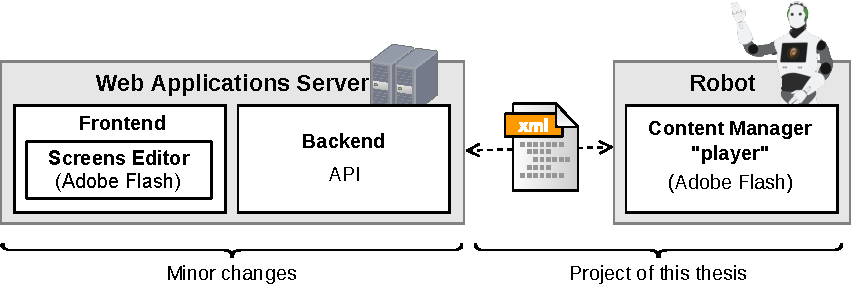
\includegraphics{figures/intro-system-overview.pdf}
    \caption{Overview of the Content Management System}
    \label{fig:intro-system-overview}
\end{figure}
More specifically, \textbf{this thesis deals with the reengineering of Flango \cm , the part of the system deployed \textbf{in the robot}} that displays content applications on the touchscreen of \reem{H} (\fref{fig:intro-system-overview}).
\textbf{It does not reengineer the rest of the system}, like the web application (that uses \flash as well) to generate content applications, although there might be minor changes to adapt their interfaces to the new technology.

It is desired not only to develop a practical solution but also to guarantee that the final output of the Flango \cm is the same that the old system generates.

This thesis is eminently a practical work, although the theoretical background has been extensively explored. 
Using web technology in a component of the robot is a novelty in the company. 
It is done to develop a sustainable product based on open standards (as opposed to the current implementation with \flash) that can be extended and reused for other robotic products that might be designed in the future.

\section{\company}
\company is a company based in Barcelona dedicated to R\&D of humanoid robots and robotic components. 
An international team of mostly mechanical, electronics and software engineers pushes forward the research on different fields, like speech recognition and generation, computer vision, walking, grasping, machine learning and navigation amongst others.
The company has developed 6 humanoid robots until 2013: \reem{A}, \reem{B}, \reem{H1}, H2 and H3, and \reem{C}.
This project targets \reem{H2} and H3, service robots with wheels and touchscreen.

\subsection*{Reem H2 and H3}
\reem{H2} (\fref{fig:reemh2}) and H3 (\fref{fig:reemh3}) are humanoid service robots featuring a screen on their torso.
They have an autonomous navigation system, speech recognition and voice synthesiser, they can find their way in different settings and help or entertain people in a friendly way.
They are intended for use in public places such as hotels, malls, airports or museums.

\begin{figure}
   \centering
   \begin{subfigure}[b]{0.4\linewidth}
       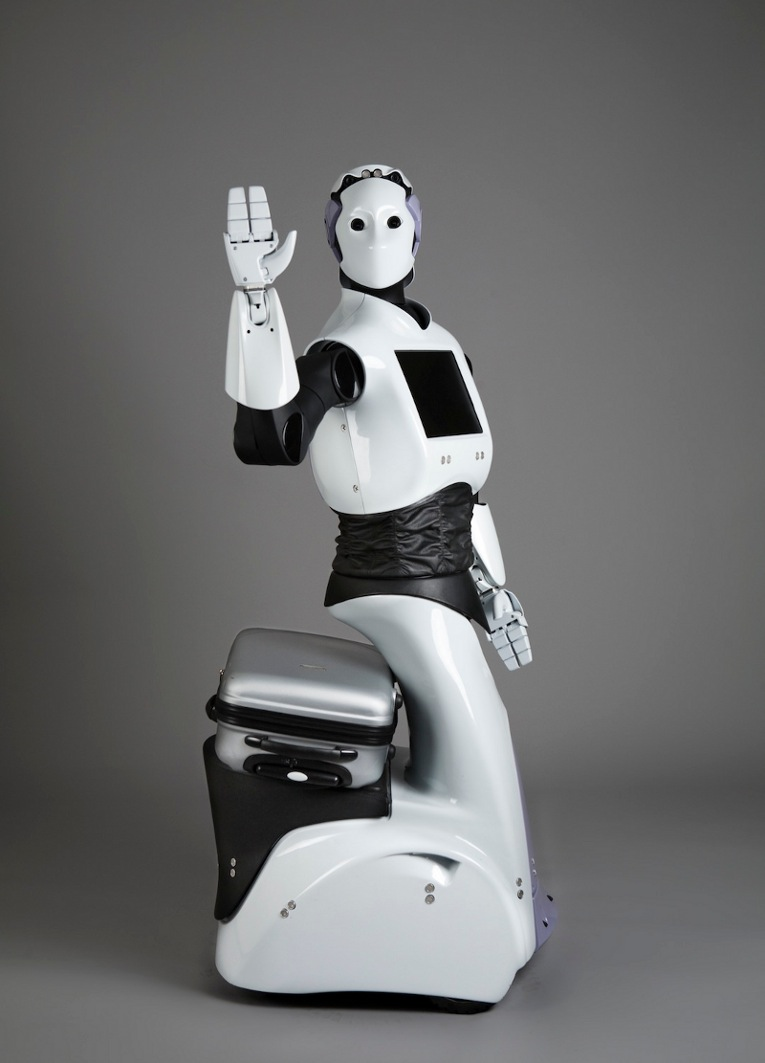
\includegraphics{figures/reemh2}
       \caption{\reem{H2}}
       \label{fig:reemh2}
    \end{subfigure}
    \begin{subfigure}[b]{0.4\linewidth}
           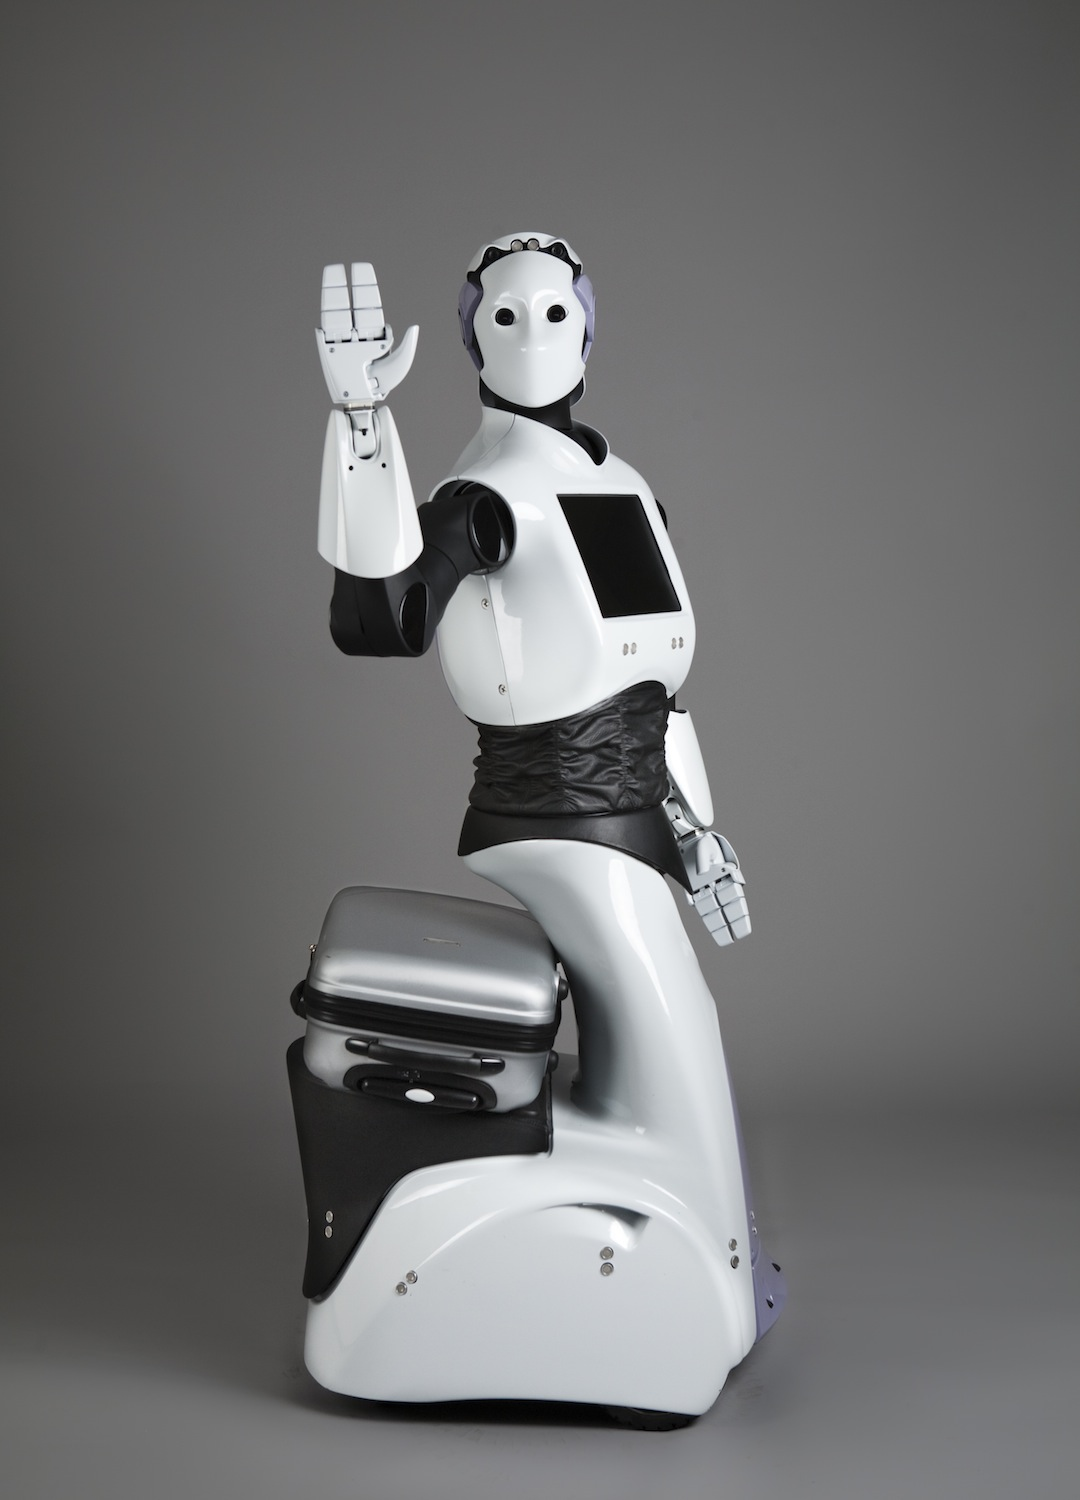
\includegraphics{figures/reemh3}
           \caption{\reem{H3}}
           \label{fig:reemh3}
    \end{subfigure}
    \caption{\reem{H} Series}
    \label{fig:reemseries}
\end{figure}
\FloatBarrier
\begin{table}
    \centering
    \begin{tabularx}{\linewidth}{| X | X |}
    \hline
    Weight & 90 Kg\\ \hline
    Height & 1.70 m \\ \hline
    Battery life & 8 h \\ \hline
    Degrees of freedom & 22 \\ \hline
    Payload & 30 Kg (mobile base), 3 Kg/arm\\ \hline
    Speed & 4 Km/h\\ \hline
    Computer & Core 2 Duo + Atom\\ \hline
    Sensors & Microphone, stereo-camera, laser, ultrasounds, accelerometers and gyroscopes\\
    \hline
    \end{tabularx}
    \caption{Reem H2 and H3}
    \label{tab:rh2}
\end{table}
\FloatBarrier
\section{The Current System}
The \reem{H} series have a multi-modal interface: besides speech or joystick manual control, humans can use a touch screen to command the robot or obtain information.
\reem{H} can display multimedia contents like videos, facts about a company, robot features, language settings, etc.

The Contents Management System comprises \emph{\flangofe} and \emph{\flangobe} (both in Basestation), and \emph{Flango \cm} (in the robot) (see \fref{fig:intro-system-overview}).
The Basestation is an application server that hosts Flango, a \ac{RIA} to manage contents and robots made with Django, a widely used framework for Python. 
Clients can create content applications  with the \flangofe (\se), a tool built with \flash .
When content applications are ready, clients can associate $1$ application with $n$ robots to display it in the touch screen.

\lstinputlisting[label=example-screen-xml,language=XML, caption={Example Screen XML}, breaklines=true]{src/example-screen.xml}

The elements of a content application (screens and entities) have an \ac{XML} representation (listing \ref{example-screen-xml}), an approach similar to popular projects (e.g. Android, NetBeans) and even, in a sense, all \acp{RIA} made with \ac{HTML}.

The Flango \cm interprets the \ac{XML} and displays the result on the screen (\fref{fig:xml-flango-view}).

A content application is essentially a set of screens, navigation, multimedia contents, and entities. 
The latter are domain objects that can be instantiated and represented in a view. 
This way a user can create an application that shows information about the company, include buttons to provide an easy way to give commands to the robot (e.g. "follow me", "shake hands"), display videos and picture galleries, etc.
All of these components are localisable:  
They can be resized, repositioned, repainted... depending on the active language.
Using other tools, clients can also associate sentences to screens and the text-to-speech system reads them aloud.

\begin{figure}[htb]
    \centering
    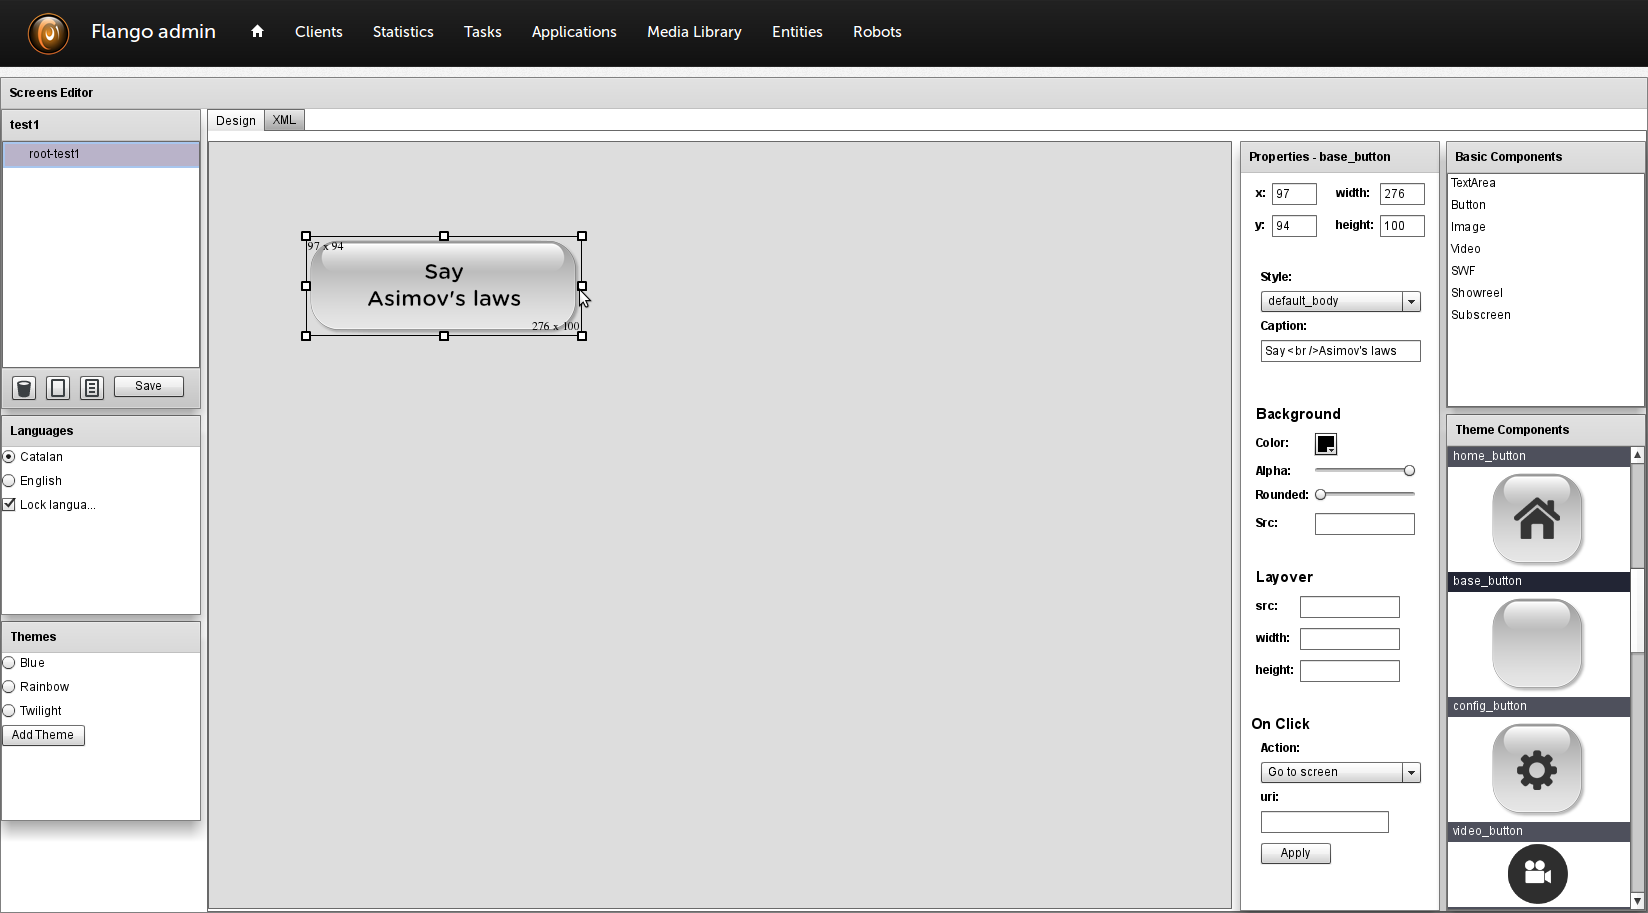
\includegraphics[width=\textwidth]{figures/screens-editor}
    \caption{\se , a \flash application in Flango}
    \label{fig:screens-editor}
\end{figure}

\reem{H} robots have a built-in software to display the content applications, the Flango \cm , which is also made with \flash .
Initially, this software has no \ac{GUI} or direct interaction with a person.
It transforms \ac{XML} files into a \ac{UI} (\fref{fig:xml-flango-view}) and, finally, displays the screens and manages the user interaction (e.g. clicks on a button).

\begin{figure}[htb]
    \centering
    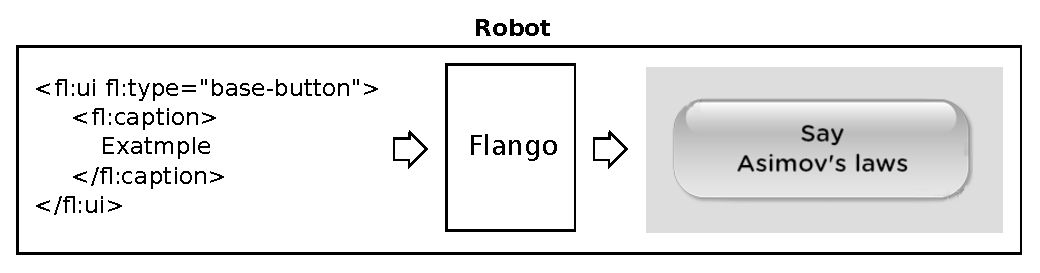
\includegraphics[width=\textwidth]{figures/xml-flango-screenshot}
    \caption{Transformation of \acs{XML} into a \acs{GUI}}
    \label{fig:xml-flango-view}
\end{figure}

\textbf{This thesis documents the project of reengineering the \cm , in the robot, with web technology instead of \flash , namely \acs{HTML5}, \acs{CSS3} and \acf{JS}}.

\section{The New System}
The \ac{WWW} was born as a document viewing platform and has evolved gradually into an application platform. 
First the web consisted of simple pages that contained structured text and some images. 
Navigation was done using simple links between pages. 
In a second phase, web sites became interactive: 
it was the time of animated graphics, browser plug-ins and JavaScript. 
More recently web sites have adopted features from traditional desktop software in \acp{RIA} \cite{Anttonen:2011}.

For a decade, the \flash player plug-in has provided a platform to enable rich and interactive content in browsers.
However, Adobe has made the updates exclusive to the Google Chrome\textsuperscript{\textcopyright}\xspace browser \cite{FlashRoadmap}. 
The browser in the robot application, QtWebBrowser, uses this plug-in but will not receive updates from Adobe. \company ' systems need to adapt to this new setting. 
There are two solutions:
\begin{itemize}
	\item Use Google Chrome instead of QtWebKit
	\item Use modern web technologies, either in QtWebKit or in another browser
\end{itemize}

The solution is rethinking the application to be a part of the robot's system and implement it with modern web technology.
There is a number of technologies that could be used, but the Web allows the product to be easily portable, very extensible, open to many developers and sustainable as it does not depend on a single company.
\ac{HTML5} is perhaps the best known forthcoming standard in the Web and is typically combined with JavaScript and \ac{CSS3}. 
It has become such a popular combination that major browser vendors provide support for the latest drafts of the \ac{W3C}, like the audio \ac{API} for \ac{HTML5} or the video support.
A big number of frameworks with JavaScript have appeared not only client-side (e.g. BackBone, jQuery, Ext JS, Google Web Toolkit, Yahoo User Interface Library...), but even server-side (e.g. NodeJS).
Moreover, new \ac{HTML5} capabilities and \acp{API} are an opportunity to add features to this project.

The project of this thesis uses Google Angular\textsuperscript{\textcopyright}, a \ac{MVC} framework that lets developers \emph{teach the browser new syntax}. 
Thus, \ac{XML} files created with the \se can be interpreted natively in a browser. 
This has some advantages over \flash \cite{Jobs:ThoughtsOnFlash}:
\begin{itemize}
    \item No use of third-party plug-ins
    \item Openness
    \item Reliability, security and performance
    \item Keeps power consumption lower (e.g. using the GPU to decode video or apply transformations and smooth transitions to elements on the screen)
    \item Touch-enabled: the new screen of Reem H3 is multi-touch. To enable gestures, heavy rewriting of the current Flash application is required.
\end{itemize}


\section{Goals}
This thesis is part of the specialisation of \emph{Software Engineering and Information Systems}. 
The goal is to reengineer the Flango \cm with web technology.
More specifically, the author has to gather the requirements from an existing system, plan in terms of scope, time and cost, make the system specifications, design and implement it using modern web technologies, use quality assurance tools and deploy it successfully in a \reem{H3} robot.

Regarding the project, the goals are:
\begin{itemize}
	\item Reengineer the current system with web technology
	\item Develop a testing strategy to make it robust
	\item Make it compatible with non-reengineered parts of the system
\end{itemize}


\section{Organisation of This Document}
This document describes the system developed at \company to display the  content applications created with the \se on the \reem{H} series.
It does not cover other software on the robots or in Basestation.

This document describes the project as follows:
\begin{description}
\item[Related Work] Provides a general overview of topics surrounding those of this thesis, enabling for a deeper understanding of the material at hand.
It starts with a description of the reengineering process, followed by a section about web technology and, finally, a description of the methodology of the project -- \ac{TDD}.

\item[Project Management] Contains information about the project from the point of view of management. 
Detailing on schedule, budget and risk analysis. Contains an assessment of the execution.

\item[Requirements] States the functional and non-functional minimum requirements, the constraints and weights the use of off-the-shelf solutions.

\item[Specification] Defines what the application does in the context of a reengineering process. 
It deals with the first three steps: a software inventory, documentation restructuring and a description of the current system (with special attention to context, interoperability and interaction).
Contains the specification of the new system: a conceptual model, use cases and the behaviour model, with sequence diagrams and contracts of system operations. 

\item[Design] Describes the internal design of the software in the context of a reengineering process. 
It contains the last three steps: code restructuring, data restructuring and forward engineering.
Detailing about the system architecture and the context and the patterns used.
Contains a static view (class and packages diagram), a dynamic view (sequence diagrams) with examples of the most relevant operations and a physical view (deployment diagrams).

\item[Implementation] Holds technical details about the environment, the set-up, the integration in the robot and a larger system and meaningful examples of the technology used. 
Emphasises the implementation of the patterns described in previous chapters.

\item[Testing] Highlights the strategy to implement tests and the integration in the robot system.

\item[Conclusion] Presents the conclusions from technical, academic and personal point of view. 
Includes challenges faced during developments and future work. FIXME

\item[Appendix A] Lists UI Components of the old system.

\item[Appendix B] Lists unit tests that define the behaviour of most components of this system.

\end{description} % intro
\chapter{Related Work}
This chapter is a short introduction to the main knowledge areas involved in the development of this project.
It describes what has been done before in the field and the theory the project is based upon.
It includes the motivation and the steps to reengineer an application , the evolution of web technology from simple documents to \acp{RIA} like the one of this thesis, the \ac{TDD} method and the relationship with \ac{DbC} and, finally, \ac{XML} as an intermediate representation of the model to interoperate between Basestation and Flango \cm in the robot.

\section{Reengineering}
\label{sec:reengineering}
This thesis takes over the work of the past two years at \company in content management.
The initial situation is a system made with \flash and Django called Flango.
The \se and the robot's \cm are \flash applications.
Whereas the first one runs in a modern browser, on desktop computers, the robot's \cm runs in the robot.
The robot is a Linux system and the browser is a QtWebKit widget embedded in the Qt application that governs the hardware.
The \flash plug-in will not be updated and this part of the system has to be rewritten in a different technology.

\begin{quote} 
Consider any technology product that has served you well. 
You use it regularly, but it's getting old. 
It breaks too often, takes longer to repair than you'd like, and no longer represents the newest technology.
What to do? If the product is hardware, you'll likely throw it away and buy a newer model.
But if it's custom-built software, that option may not be available. 
You'll need to rebuild it. 
You'll create a product with added functionality, better performance and reliability, and improved maintainability.
That's what we call reengineering. \cite{Pressman:2007}
\end{quote}
Unlike other products, software does not degrade with time due to external factors such as the inclemencies of the weather, power outages or intense use.
Software packages are adapted, corrected, extended and improved constantly.
That can lead to unstable applications or unexpected side effects, even if the original product had been designed with the best practices at that time.
After a certain amount of time, changes are harder to implement. % FIXME language
Sometimes the vendor of frameworks, libraries and third-party software used in a project stops supporting it and the only solution is substituting the components that depend on it. 
The product becomes unmaintainable in many aspects and reenginering is required. 

Software reengineering comprises \textbf{6 activitie}s: \textbf{inventory analysis}, \textbf{document reestructure}, \textbf{reverse engineering}, \textbf{code restructuring}, \textbf{data restructuring} and \textbf{forward engineering}.
Simple put, it is all about understanding the current logic of a program and modifying the three typical components: data, logic and view.
The project of this thesis is not modifying the current program but developing a new one with new technology, focusing on reverse engineering the original software. 

Doing an inventory of the software that belongs to the system is part of the definition of the project scope.
Making a list of programs with the current status, dependencies and physical location helps on getting an overview of the project.
Usually software has documentation that needs to be added to the inventory and, sometimes, restructured.
After this, the reverse engineering process can start.

\paragraph{Reverse Engineering}
Three dimensions drive tasks in the reverse engineering activity (FIXME task in activity or the other way round?): abstraction level, completeness and directionality.
To understand what the software does, abstraction should be as high as possible.
This information can have many details or not (completeness) and can be created in one way (extracting it from the source code) or two-way (feed information to the reengineering tool).
This project does not use any computer-assisted reengineering tool.

\subparagraph{Understand current program}
A program normally has input data, logic that processes it and a view:
The first activity is understanding the processing.
Code can be examined at several levels of abstraction: system, program, component, pattern, statement.
Some key aspects include the interaction, interoperability or the context.
Data structures, classes, schemas in databases, etc have to be identified and possibly redesigned in the next steps.
Finally, the \ac{UI} has to be analised as well. 
There are issues related to presentation of data, interaction, usability, etc that have to be identified.
This project focuses on system and program levels of abstraction and on interoperability.
The software does not have any views or databases to be reconsidered.
However, it does have some formats server-side (in the backend) that are candidates in this process (e.g. definition of settings with \ac{XML} might have to become \ac{JSON} or have a different structure).

\paragraph{Restructure code and data}
Sometimes the solution is restructuring the current program.
The project of this thesis skips this part because a new application is being developed using the output of the first activity (FIXME: activity?): understand the current program
Restructuring the code might not be enough in most cases. 
It can fix immediate issues but it is not a long-term solution.
However, when doing so, \ac{TDD} is useful because tests breaks immediately and often, specially if they are running in the background or periodically.
To improve the software design both data and architecture should be restructured.
\ac{TDD} can provide robustness to this process: if there are tests available, the new design can be proven to work, at least, for the example cases. 
If not, the solution can be built incrementally with tests that define the requirements of the system (extracted in the first activity (FIXME: activity?), thus using them as an specification.

\paragraph{Forward engineering}
There is a number of options when it comes to apply changes in the current program. 
For example, apply patches, redesign parts of the software or completely redesign it.
Depending on the circumstances, completely redesigning a software might be costly but, in the long-term, it might be a cost-effective solution.
The project of this thesis is redesigning the software to incorporate new practices, new technology and, in the future (out of the scope of the thesis), additional requirements.
The outcome of this process (FIXME process vs activity vs task) is a new software that replaces the current implementation.

%introduction

%software reenginering:
%main activities (software reengineering prcess model defines 6 activities, fig 30.2):
%inventory analysis
%document reestructure (option 1)
%reverse engineering
%code restructuring
%data restructuring
%forward engineering

%reverse engineering:
%keys: abstraction level, completeness, directionality:
%abstraction: make it as high as possible (ideally, entity-relationship models)
%completeness: how much detail prvided at an abstraction level?
%(there are tools to analyse software but this thesis isn't using them)
%directionality: one way. extract info from the source code, give it to an engineer, use it during any mmaintenance %activty,. it can also be two-way (feed info to a reengineering tool that fixes the old program)

%first activity of reverse engineering: understand processing. analyse code at varying levels of abstraction: system, %program, component, pattern, statement. 
%understand overall functionality before doing more steps (set a context, pay attention to interoperabilty issues). %Block diagrams of the programs (show interaction). do some narrative for each component.
%normally there is code for: prepare data, process data, prepare results for the view

%next activity: understand data:
%internal data structures. goal: identify classes. focus on teh definition of classes of objects. book is old-fashioned %and assumes crappy old code.
%database structure. bottomline: rethink the design.

%next: reverse enginer UI

%restructuring
%(mention it. this is related to TDD)
%code restructuring is not enough. it alleviates immediate problems. real benefit is achieved only when data and %architecture are restrucured. spaguetti-bowl code to structured programming.
%data restructuring: standarise, rationalise, make physical modifications.

%forward engineering: change the code, redesign, or make big changes (completely redesign, recode, test..). preventive %maintenance. cost of maintenance.


\section{Web Technology}
% quotations: something about emacs life style, or berners lee
The \ac{WWW} plays a central role in many people's lives.
The first drafts date back to the 1980s, the first web browser prototype by Tim Berners-Lee was built in December 1990 and the Mosaic browser was completed in 1993.
After that, Netscape, Mozilla Firefox, Microsoft Internet Explorer, Google Chrome, Safari, Opera, Konqueror and many other browsers appeared, along with some nowadays popular websites (e.g. Amazon, 1995).

For many people the browser is the most used application in many devices. 
The web creates opportunities and makes documents accessible like tax records, maps, banking information, phone directories or product catalogues.
New business models, like new ways of promoting products, selling music or movies, are developed having the web as a core part.
Innovation goes beyond all these with experiments and products like FirefoxOS or ChromeOS to build an operating system where the web is the main development platform.
Other companies, like Citrix or eyeOS, offer web applications or virtualisation tools that resemble an operating system %\cite{Gamonal:2011}.

%goals: explain evolution of web tech, state of the art, and why it is better than flash.

%* programs in browsers. isolate them? flash plugin. flash is dead (jobs or other
%articles) 
%* browsers: architecture (dom, js engine, html renderer...) from mosaic to
%%fx/ch/qtwebkit 
%** webkit and qtwebkit
%
%* client-side tech: JS, css, html/xml 
%** evaluation and comparison 
%** frameworks
%
%browsers, JS engines, chrome v8, fx gecko, QtBrowser
% functionaliyy (interoperability, security), reliability (maturity), usability: (learn-
%ability, attractiveness) Efficiency: (time behavior, resource utilization) Maintainabil-
%ity: (stability) Portability: (installability)

\subsection{From Plain Documents to Applications}
\paragraph{The Evolution of the Web}
\begin{quote} 
HyperText is a way to link and access information of various kinds as a web of nodes in which the user can browse at will. 
Potentially, HyperText provides a single user-interface to many large classes of stored information such as reports, notes, data-bases, computer documentation and on-line systems help\cite{BernersLee:1990}
\end{quote} 

When the \ac{WWW} was started in 1990 it was intended to be a document viewing platform.
It has evolved in at least three phases \cite{Anttonen:2011} \cite{Taivalsaari:2008}:

In the early days, websites were basically a few files with plain text, forms and page-structured artifacts, possibly static images and hyper-links (anchors) to provide navigation. 

Later on, browsers added programming capabilities, plug-ins and allowed animated graphics. 
Web pages became interactive and client-server communication increased in complexity.
\flash (at that time Macromedia Flash), ShockWave, Java, QuickTime and a few others allowed the inclusion of multimedia contents or even programs (e.g. Java Applets).
Engineers could combine server-side and client-side technology to provide some more capabilities along with content.

More recently, despite the fact that the web browser was not designed for running applications, since 2008 users have headed this way. 
In this third phase, web pages are not just documents: they have complex user interaction capabilities, they do not require full page refresh and typical use cases have evolved. 
A big part of applications is executed client-side, taking advantage of the computing capabilities of modern hardware and decreasing the load in servers. 
In some cases, the application also needs huge server-side resources and uses strategies like cloud computing (e.g. Amazon EC2) to scale up.
Today the web is not only about viewing documents but about world-wide sharing, collaboration and interaction, possibly in real time. 

Web browsers have become a widely-used platform for software applications. 
Video editors, spreadsheets, calendars or 3D games used to run exclusively on desktop computers. 
Today, they run in a variety of devices and some of them even do it in a browser. 
There are 3D engines ported to Web, real time collaboration, full HD video support without plug-ins and many more features built-in a system, the browser, that is not an ideal execution environment for desktop applications.

\paragraph{\ac{RIA}}
\acp{RIA} are neither web services or web pages. 
They are software systems based on technologies and standards of the \ac{W3C} that provide web specific resources such as content and services through a web browser \cite{Kappel:2006}.
Typically one designs them as single page websites.

% FIXME language
Web applications differ between them. 
They can be document-centered, workflow-based, portal-oriented, collaborative, social, etc. 
They all have some common characteristics. 
Amongst others:
\begin{itemize}
    \item The product
    \begin{itemize}
        \item Content is the core.
        \item Hyper-text: non-linearity is a main distinction to traditional software systems. There are many ways of landing on a certain page. This can lead to disorientation or cognitive overload for users.
        \item Presentation aesthetics, usability and interaction are closer to a desktop application than to a web page
    \end{itemize}
    \item Use
    \begin{itemize}
        \item Globality: Spontaneity and multiculturality of users. Web applications are publicly available.
        \item Quality suffers from unknown network characteristics
        \item Multiplaform delivery involves having different devices, browsers and degrees of functionality and performance
        \item Intense network usage. Remote calls are minimised. The use of software patterns like remote facade, remote proxy, \ac{DTO} or \ac{RPC} is frequent
    \end{itemize}
    \item Evolution
    \begin{itemize}
         \item Continuous change
         \item Competitive pressure
         \item Fast pace development
    \end{itemize}   
\end{itemize}

The project of this thesis is, in a sense, both a \ac{RIA} and a \acp{RIA} generator. 
It is a \ac{RIA} because, among other reasons, it works in the browser with web technology and has an intense use of the network to fetch the model or other components to build the screens.
The rendered application works in a browser, has an intense use of the network as well and is content-centered.
Despite the fact that it works in the specific content of a robot, globality is still an issue.
A typical scenario would be a fleet of robots in a conference: users from many different cultural backgrounds can use the application at any time.


\subsection{Browsers and isolation of programs}    
Many of the websites in the aforementioned third phase contain substantial amounts of client-side code. 
At the end of the day, a \ac{RIA} is a distributed software. 
In the past the client-side part was thin and simple, whereas today's application have complex logic delegated to client nodes with local storage, hardware-accelerated components, websockets and other advanced capabilites.

In spite of the fact that \acp{RIA} have grown in complexity and now demand more resources, browsers architectures still do not provide sufficient isolation between concurrently executing programs.
A similar problem occurred in early operating systems (e.g. MS-DOS), before processes appeared \cite{Reis:2009}. 

Most of browsers have a monolithic architecture with poor isolation between web application instances. Chromium, however, implemented an architecture based on \ac{OS} processes. 
Another way of isolating web applications is running them in a plug-in container. 

The project of this thesis does the first phase with Qt WebKit, the port of WebKit on top of Qt, to display the application in a Qt dialog and communicate with the hardware. 
The second part uses Chrome to meet the technology requirements.
Qt WebKit components comprise the WebCore and SquirrelFish Extreme, which compiles Javascript into native machine code. 
It is compatible with Adoble Flash Player but because it will not receive more updates in the future, it will not be used any more.
The \flash plugin is a black box isolated from other elements in the \ac{DOM}.
Isolation is not an issue in this project because there is only one application running at a time and, even in a normal use of a browser, with many websites running at once, isolation is not a blocking issue.
FIXME MAYBE ADD CHROME V8 engine, ETC.

% MOVE THIS TO DESIGN
%\section{Client-side Technology}
%The software of this thesis is developed mainly on the client side and is part of a Web system.
%There is a number of technologies to develop applications client side. 

%\subsection{Comparison of languages}
%\subsection{Frameworks}

\section{Test-Driven Development}
The software written for this thesis is executed in a complex environment.
Testing it properly and ensuring the quality is crucial to avoid unexpected behaviour in one of the most visible parts of this system, the screen.
Crashes and \ac{UI} flaws can lead to triggering wrong external calls to other components of the system (e.g. displaying a Qt dialog different than expected, not making the call, sending it with bad parameters...), blocking access to features or seriously affecting the \ac{UX}.

Reengineering this system has, at least, two sources of potential errors: 
undocumented features in the original application (unknown, documented wrongly, partially documented or not described at all) and integration of the new software in the current system.

% maybe put all this in a table?
\ac{TDD} is based on having numerous and very short iterations with these steps:
\begin{enumerate}
    \item Add an initial (failing) test
    \item Run all tests and see if the new one fails
    \item Write the minimum amount of code to pass the test
    \item Run the automated tests and see them succeed
    \item Refactor the code. Conform to standards and best practices
\end{enumerate}

As opposed to classic development methodologies (e.g. waterfall, where tests are done in the last place), with \ac{TDD} tests go first. 
Specification and documentation of the system are not artifacts created before the implementation but the tests themselves.

Testing earlier and heavily has benefits over the classical approach:

\textbf{Efficiency} Defects (and their causes) are identified earlier.

\textbf{Robustness} The system is more reliable and stable. 
The \ac{QA} process is easier to maintain and much more strict.

\textbf{Maintainability} Small fixes can introduce new errors in the system. 
Testing continuously and producing the minimum amount of code to implement a feature reduces this.

\textbf{Extensibility} \ac{XP} embraces change. 
It is easier to adapt to changes in the requirements. 
This thesis is reengineering a project that is not frozen. 
During the development, the original software keeps adding features and bug fixes.

This methodology is specially useful in the implementation of this project for two reasons: 
the Google AngularJS framework is extremely friendly with unit testing and \ac{E2E} tests thanks to Karma Runner, and the company has the infrastructure to incorporate the project in a continuous integration system with Jenkins.

\section{XML as an intermediate representation}

lorem ipsum
 % related work
\chapter{Project Management}
This chapter describes the planning of this project in terms of scope, schedule, cost and risk.
The execution and deviations are shown at the end of this chapter.

\section{Scope}
\label{sec:scope}
The system has three parts: the \flangobe, the \flangofe (with the \se) both at Basestation, and the screens renderer in the robots (the robot's \cm \fref{fig:system-overview}).

\begin{figure}[htb]
    \centering
    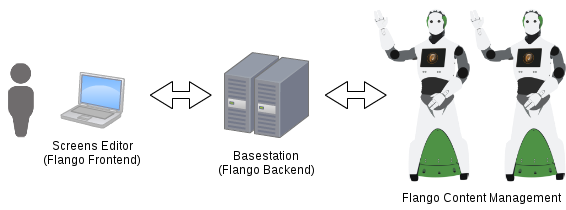
\includegraphics[width=14cm]{figures/intro-system-overview}
    \caption{System components}
    \label{fig:system-overview}
\end{figure}

This project reengineers the robot's \cm with web technologies but not the back-end and front-end, that remain in Django and \flash.
The input of the new \cm are contents applications, generated with the \se . The output is the screen rendered with web elements.
Contents applications have configuration files that define the theme, the location of binary resources (images, videos, etc), the default language and other settings. 
This project can read and use the configuration files.
This project accepts valid syntax generated with the \se for a comprehensive set of components (\texttt{back-button}, \texttt{base-button}, \texttt{image}, \texttt{video}...) and their properties (\texttt{width}, \texttt{x}, \texttt{y}, \texttt{background}...), and generates \ac{HTML5} that renders them as defined.

Developing an intense testing strategy is part of this project.
The final artifact is this master thesis that describes the system and the rationale that guides all decisions.

\section{Schedule}
This project has 4 phases that match the 4 typical groups of processes: initiating, planning, executing (and monitoring + control) and closing.
The execution has 3 deliverables: viability and proof of concept, iteration 1 (basic program) and iteration 2 (extended program).

\subsection{Phase 1: Initiating}
\paragraph{April, 1 -- April 4}
The initiating processes determine the goals of the project and the scope.
This stage was partially done before the beginning of this thesis to ensure its viability in the company.
It was agreed that the project would reengineer the current system using web technologies (see \fref{sec:scope})

\subsection{Phase 2: Planning}
\begin{sidewaysfigure}[htb]   
    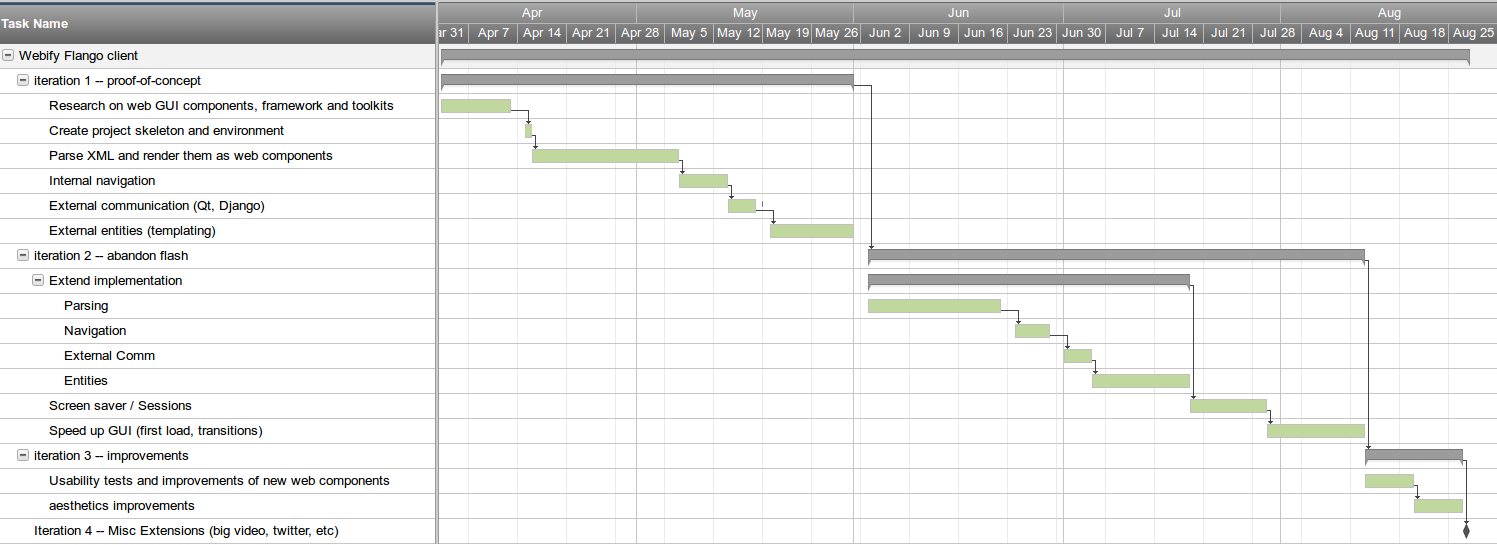
\includegraphics[width=\textwidth]{figures/plan-gantt-orig}
    \caption{Original Gantt Chart}
    \label{fig:plan-gantt}    
\end{sidewaysfigure}

\paragraph{April, 5 -- April 6}
The first draft of the plan is a rough estimation of the tasks length and a definition of the big milestones.
Because there is only one engineer there are no concurrent tasks and free floats are always zero.
Other activities of this phase include an estimation of the resource requirements for upcoming tasks, developing the budget (\fref{sec:budget}) and risk planning (\fref{sec:risk}).
See the Gantt chart in \fref{fig:plan-gantt}.

\subsection{Phase 3: Execution}
\paragraph{April, 7 -- August 28}
The execution phase focuses on building the product. 
A web engineering process should be incremental, with frequent changes and short iterations \cite{Kappel:2006}.

\begin{table}[htb]
    \centering
    \begin{tabular}{| l | p{11cm} |}
    \hline
    Milestone & Deliverables \\
    \hline
    Proof of concept & Research on frameworks and tools to develop the project. Choose one. Build a minimal working example to illustrate key aspects of the project. \\ \hline
    Iteration 1 & Build a prototype comprehensive in number of features but simple in the implementation to validate the technology. \\ \hline
    Iteration 2 & Extend the prototype of Iteration 1 to complex cases. \\
    \hline
    \end{tabular}
    \caption{Milestones and deliverables of the execution phase}
    \label{tab:milestones}
\end{table}

This phase has 3 big milestones, one per iteration (\fref{tab:milestones}). 
The outcome of each iteration is a product with a set of stable features and the corresponding unit tests which, in turn, serve for the purpose of documentation.

\subsection{Phase 4: Closing}
\paragraph{August, 29 -- September 14}
Prepare package with a stable set of features, presentation and documentation.

\FloatBarrier

\section{Cost}

\FloatBarrier

\label{sec:budget}
The estimated length of the project is $105 days \times 8 \euro{} \times 8 hours = 6720 \euro{} $

\begin{table}[ht]
    \centering
    \begin{tabular}{| l | l |}
    \hline
    Labour & 6720\euro{} \\ \hline
    \multirow{3}{*}{Hardware} 
        & Desktop Computer (amortized) 250\euro{} \\ % check this
        & 22 Monitor (amortized) 50\euro{} \\
        & Reem H3 testing time 150\euro{} \\ \hline   
    \multirow{2}{*}{Software}
        & JetBrains WebStorm license 89.10\euro{} \\ % check this    
        & GNU/Linux 0\euro{} \\ \hline
     Overall & 7259.10\euro{} \\ 
     \hline
    \end{tabular}
    \caption{Budget}
    \label{tab:budget}
\end{table}

There are some infrastructure related costs excluded from the budget because they are part of the office maintenance monthly expenses.
This is the case of subversion servers, network, power, backups, etc. 

\section{Risk Analysis}
\label{sec:risk}
\begin{risk}
{Schedule: deviation}
{There might be urgent needs in the company, like demos to potential customers or hot bugs related to contents applications}
{Some of the needs are unpredictable. However, preventive maintenance and good documentation of bugs in tickets can reduce the chances that this risk will occur.}
{Do the urgent task and reschedule the project}
\end{risk}

\begin{risk}
{Resources: deviation}
{The engineer might have to dedicate resources to other tasks in the company non-related to this project.}
{Coordinate action monthly with the managers and track deviations and progress weekly. Avoid dedicating less than 50\% of time to this project.}
{Limit scope and extend deadlines to have the expected number of hours dedicated to this project.}
\end{risk}

\begin{risk}
{Resources: infrastructure crash}
{The development system might die}
{Use version control systems and do frequent and small commits. Delegate backups to the IT team.}
{Restore backups}
\end{risk}

\begin{risk}
{Resources: testing environment not available}
{Most of the testing can be done with regular computers. However, final tests have to be conducted with real hardware: ReemH3-1 or 2 and Reem-H2, which are frequently booked to go on tour, perform shows, demos or development.}
{Book 3 days in advance if testing is critical. }
{Share the robot with a team that doesn't need the media computer of the robot, where this project is hosted.}
\end{risk}

\begin{risk}
{Personnel: Application expert leaves the project}
{There is only one application expert that can leave the company. Nobody else has advanced knowledge on the internals of the current implementation.}
{Build a common agenda with the expert and document critical and complex parts of the current application. Find experts in similar technology in the team}
{Reach him on-line, hire him as consultant, take conflicting features out of the scope of the project.}
\end{risk}

\begin{risk}
{Quality: critical use cases not implemented}
{One or more critical use cases can not be implemented}
{Verify that the technology allows implementing them. Build a prototype. }
{Find a workaround. Assess the importance of the affected use cases and adapt to change: decide if changing the specification of the use case will fix this.}
\end{risk}

\begin{risk}
{Quality: look and feel of the current theme can't be implemented}
{The current look and feel and interaction is designed for Adobe Flash. It might not suit the way web technology works.}
{Verify that the technology allows it with a prototype.}
{Change the external design to balance the needs of the technology and the customer}
\end{risk}

\begin{risk}
{Scope: Non-intuitive implementation with web technology}
{Current implementation is designed for Adobe Flex. Some of the use cases to implement might not fit well with the new technology}
{Analyse and discuss use cases with the author of the old implementation}
{Explore ways to change the implementation of the use case in the Screens Editor (which generates the input for the new program) to fit in the new design}
\end{risk}

\begin{risk}
{Inadequate technology}
{The chosen technology is inadequate: it doesn't allow a complete reengineering of the application (100\% of chosen use cases), performance is more than 10\% lower, it is not reliable and fails in more than 3\% of action executions}
{Assess at least 2 solutions before implementing a prototype. Implement a prototype with basic cases of at least each critical feature.}
{sdnsdgndf}
\end{risk}

\begin{risk}
{Tool: Flango or \se do not perform as advertised}
{The current implementation of the backend or the screens editor might have bugs.
Some undocumented features or \ac{XML} elements might be misleading (e.g. The normal behaviour for the QR component is generating a QR code. \lstinline$<ui type="qr" src="path">$ does not generate a QR code, but embeds an image that already exists instead.) }
{Contact the application expert before implementing the feature.}
{Fix the backend (python) or ask/hire the application expert to fix the screens editor (Adobe Flash)}
\end{risk}

\begin{risk}
{AngularJS or dependencies do not perform as advertised \footnote{Added after specifications were defined}}
{The chosen framework and libraries have young maturity and might contain bugs, be subject to rapid changing cycles and new versions might break older versions}
{Use stable versions}
{Investigate the bug, isolate it, create a minimal full working example and, if possible, open a pull request with a fix in Github or notify the error to the project managers.}
\end{risk}

\FloatBarrier

\section{Execution}
progress, deviations, final cost
FIXME % plan
\appendix
%\chapter{Tables}

\begin{table}
\caption{Armadillos}
\label{arm:table}
\begin{center}
\begin{tabular}{||l|l||}\hline
Armadillos & are \\\hline
our	   & friends \\\hline
\end{tabular}
\end{center}
\end{table}

\clearpage
\newpage

%\chapter{Figures}

\vspace*{-3in}

\begin{figure}
\vspace{2.4in}
\caption{Armadillo slaying lawyer.}
\label{arm:fig1}
\end{figure}
\clearpage
\newpage

\begin{figure}
\vspace{2.4in}
\caption{Armadillo eradicating national debt.}
\label{arm:fig2}
\end{figure}
\clearpage
\newpage

%% This defines the bibliography file (main.bib) and the bibliography style.
%% If you want to create a bibliography file by hand, change the contents of
%% this file to a `thebibliography' environment.  For more information 
%% see section 4.3 of the LaTeX manual.
\begin{singlespace}
\bibliography{main}
\bibliographystyle{plain}
\end{singlespace}

\end{document}

